\documentclass[twocolumn,twoside]{base/jrekpros}
\usepackage[switch]{lineno} % Display line numbers; comment this and \linenumbers out when finalising

% Article information (authors ignore)
\articleinformation{VOLUME xx, NUMBER x, xxxx, xx–xx} % Volume, issue, year, page range
\articleinformationtruncated{xx(x): xx–xx} % Truncated volume, issue, page range
\articledoi{\href{https://doi.org/10.22146/jrekpros.xxxxx}{10.22146/jrekpros.xxxxx}} % Article DOI
\articletype{ARTICLE TYPE} % Article type
\submitted{1 Month 2000} \revised{1 Month 2000} \accepted{1 Month 2000} % Article genesis

% Article title
\title{The \textit{Jurnal Rekayasa Proses} \LaTeX \,template, for use in typesetting manuscripts and preparing submissions}

% Author(s)
\author[1,*]{First Author}
\author[2]{Second Author}
\author[2]{Third Author}

% Corresponding author's email address
\email{email@address.com}

\authorheader{Author et al.} % Author name(s) as they should appear in the header

% Author(s) affiliations
\affil[1]{First author's affiliation. Provide the full postal address, including street name and number, city, ZIP code, and country}
\affil[2]{Second and third authors' affiliation. Provide the full postal address, including street name and number, city, ZIP code, and country}

\begin{document}

\setcounter{page}{1}

\maketitle
\thispagestyle{firststyle}
\linenumbers % Add line numbers

{\centering\frame{
\includegraphics[width=1\linewidth]{figures/abstract-image.jpg}}} % Abstract image goes here; "\frame" adds a frame around the image

\begin{abstractcontent} % Add abstract and keyword content here

{\objective} Articles in English only need to have an English abstract. Briefly state the objectives of the research. {\methods} List the methods used in the research. {\results} Briefly describe your principal results. {\conclusions} State your conclusions here.

{\keywords} alphabetical order; maximum five keywords; avoid terms already in the title

\end{abstractcontent} % End of abstract and keyword content

\section{INTRODUCTION}

This section should briefly explain the background of the study, provide a short review of the pertinent literature, state the originality or novelty of the research, and state the research objectives. This is an \textit{example} of \textit{italicized} text (\textit{The quick brown fox jumped over the lazy dog.}); \textbf{don't use bold text} unless it is called for by the content. 

\section{MATERIALS AND METHODS}

In research articles, the materials and methods used in the study should be described together—first the materials, and then the methods. Enough information should be provided to enable repetition of the research. For commercial sources of the materials, the name of the company, and the town and country in which they are headquartered should be indicated. To avoid an excessively long methods section, methods that have already been published should be indicated with a reference, with only the relevant modifications described.

\subsection{Equations}

Equations should be directly referenced in the text, and typeset using the available \LaTeX\, commands (Equation \ref{eq:1}).

\begin{equation}
    J(x) = Li(x) + \sum_\rho Li(x^\rho) - \text{log}\,2 + \int^\infty_x \frac{dt}{t(t^2 - 1) \text{log}\,t}
    \label{eq:1}
\end{equation}

\noindent Long equations can use the \verb|aligned| environment to make them fit in a single column (Equation \ref{eq:2}).

\begin{equation}
    \begin{aligned}
        J(x) &= Li(x)\\ &+ \sum_\rho Li(x^\rho)\\ &- \text{log}\,2\\ &+ \int^\infty_x \frac{dt}{t(t^2 - 1) \text{log}\,t}
    \end{aligned}
    \label{eq:2}
\end{equation}

\subsection{Lists}

This is an ordered list:

\begin{enumerate}
    \item First item,
    \item Second item, and
    \item Third item.
\end{enumerate}

\noindent Please do not use unordered lists.

\section{RESULTS AND DISCUSSION}

Combine the results and discussion in a single section. Describe the results first, presenting all data as concisely as possible in the form of tables or figures (if appropriate). 

The discussion should be an interpretation of the study's results in the context of previous research. Avoid simply repeating the results, or excessive citations. Instead, the works being cited should be relevant to the results being discussed.

\subsection{Tables}

Size a table to fit in a single column (Table \ref{tab:1}) or across two columns (Table \ref{tab:2}). Avoid large tables (i.e. those that fit more than a single page), unless absolutely necessary; otherwise, consider making them supplementary material. Table \ref{tab:3} shows various advanced options you can use, as well as the best practices for alignment, both horizontally and vertically. Note also that sentence case is used for headers (``Left-aligned column" not ``Left-Aligned Column").

All tables and figures should be cited in the text, in numerical order (Table 2 cannot be cited before Table 1). Place table footnotes below the table, indicating them with superscripted lowercase letters or asterisks (for significance values and other statistical data).

\subsubsection{Table captions}

Every table should have a caption that is concise but clear enough to explain its main components independently of the text. Use sentence case. If the table contains previously published material, cite the original source at the end of the caption. If the results are expressed as a percentage, state the absolute value(s) that correspond to 100\%.

\begin{table}[t]
  	\centering\footnotesize\sffamily
  	\caption{Example single-column table.}
  	\begin{tableminipage}{\linewidth}
    	\begin{tabularx} {\linewidth}{XXX}
			\toprule
            Column 1\textsuperscript{a} & Column 2 & Column 3  \\            
	    	\midrule
            Row 1 & Row 1 & Row 1 \\
            Row 2 & Row 2 & Row 2 \\
            Row 3 & Row 3 & Row 3 \\
            Row 4 & Row 4 & Row 4 \\
            Row 5 & Row 5 & Row 5 \\
            \bottomrule
    	\end{tabularx}
        \label{tab:1}
        \vskip0pt
        \textsuperscript{a}Example footnote.
  	\end{tableminipage}
\end{table}

\begin{table*}[b]
  	\centering\footnotesize\sffamily
  	\caption{Example double-column table.}
  	\begin{tableminipage}{\linewidth}
    	\begin{tabularx} {\linewidth}{XXXXXX}
			\toprule
            Column 1 & Column 2 & Column 3 & Column 4 & Column 5 & Column 6 \\
	    	\midrule
            Row 1 & Row 1 & Row 1 & Row 1 & Row 1 & Row 1 \\
            Row 2 & Row 2 & Row 2 & Row 2 & Row 2 & Row 2 \\
            Row 3 & Row 3 & Row 3 & Row 3 & Row 3 & Row 3 \\
            Row 4 & Row 4 & Row 4 & Row 4 & Row 4 & Row 4 \\
            Row 5 & Row 5 & Row 5 & Row 5 & Row 5 & Row 5 \\
            \bottomrule
    	\end{tabularx}
        \label{tab:2}
  	\end{tableminipage}
\end{table*}

\begin{table*}[b]
    \vspace{-6pt} % Remove some vertical space if necessary
  	\centering\footnotesize\sffamily
  	\caption{Example of advanced table options. Left-aligned columns are useful for text-only columns, and center-aligned columns for centering numbers. The X option tells \LaTeX{} to space the column(s) evenly.}
  	\begin{tableminipage}{\linewidth}
    	\begin{tabularx} {\linewidth}{lcrXXp{3cm}}
			\toprule
            Left-aligned column & Center-aligned column & Right-aligned column & \multicolumn{2}{c}{Multicolumn heading} & Column set to a specific \newline dimension \\
            \cmidrule{4-5}
            & & & Multicolumn 1 & Multicolumn 2 & \\
	    	\midrule
            Left-aligned row 1 & Center-aligned row 1 & Right-aligned row 1 & Row 1 & Row 1 & Row 1 \\
            Left-aligned row 2 & Center-aligned row 2 & Right-aligned row 2 & Row 2 & Row 2 & Row 2 \\
            Left-aligned row 3 & Center-aligned row 3 & Right-aligned row 3 & Row 3 & Row 3 & Row 3 \\
            Left-aligned row 4 & Center-aligned row 4 & Right-aligned row 4 & Row 4 & Row 4 & Row 4 \\
            Left-aligned row 5 & Center-aligned row 5 & Right-aligned row 5 & \multicolumn{2}{l}{Example multicolumn row (left-aligned)} & Row 5 \\
            \bottomrule
    	\end{tabularx}
        \label{tab:3}
  	\end{tableminipage}
\end{table*}

\subsection{Figures}

Ensure that the figure will fit into either one column (Figure \ref{fig:1}) or two columns (Figure \ref{fig:2}). Images should be of sufficiently high resolution to be easily viewable when printed or on high resolution screens (minimum of 300 dpi).

Every figure should be cited in the text, in numerical order. Figures should be referred to as "Figure" not "Fig." Denote figure parts with lowercase letters (e.g. Figure \ref{fig:3a}, Figure \ref{fig:3b}).

\subsubsection{Figure formatting}

Photographs must have internal scale markers and symbols, and arrows or letters should contrast greatly with the background. \href{https://www.fontsquirrel.com/fonts/aller}{Aller} is our recommended typeface for text within figures; otherwise, close approximations such as
\href{https://www.fontsquirrel.com/fonts/agane}{Aganè}, \href{https://www.fontsquirrel.com/fonts/merriweather-sans}{Merriweather Sans}, or \href{https://www.fontsquirrel.com/fonts/amble}{Amble} should be used. Where photographs of gel, autoradiograms, etc., have been processed to enhance their quality, this should be stated.

\subsubsection{Figure captions}

Every figure should have a caption that is concise but clear enough to explain its main components independently of the text. If the figure contains previously published material, cite the original source at the end of the caption.

\begin{figure}[t]
	\centering
	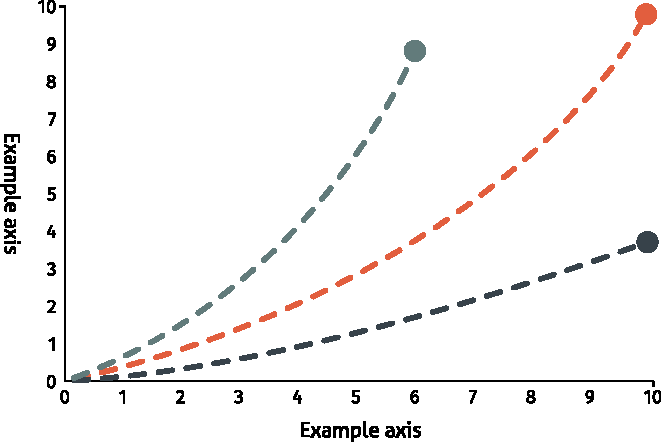
\includegraphics[width=\linewidth]{figures/figure-1.pdf}
	\caption{An example chart. Charts, illustrations, and other images that are readable in a single column should be typeset as single-column figures.}
	\label{fig:1}
    \vspace{0pt} % Add some vertical space if necessary
\end{figure}

\begin{figure*}[t]
	\centering
	
\includegraphics[width=\linewidth]{figures/figure-2.jpg}
	\caption{And example double-column figure. Charts, illustrations, and other images that are wider than they are tall might be more readable as double-column figures, whereas tall images will likely take up too much page space.}
	\label{fig:2}
\end{figure*}

\section{CONCLUSIONS}

Present the main conclusions of the study, along with their implications for future research here.

\section*{ACKNOWLEDGMENTS}

Acknowledge anyone who contributed to the research or the writing of the manuscript, as well as any funding or grants received in support of it. Funding organizations' names should be written in full, along with the grant numbers, if available. Examples of individuals you should acknowledge include those who provided assistance with study design or analysis, guidance through a study area, or who provided advice on the language, edited, or proofread the article.

\section*{AUTHORS’ CONTRIBUTIONS}

Each author’s contribution to the research and manuscript should be noted, using only their initials to indicate their names. For example, ``FA, SA designed the study. SA, TA carried out the laboratory work. FA, SA, TA analyzed the data and wrote the manuscript. All authors read and approved the final version of the manuscript."

\begin{figure}[!b]
    \centering
    \captionsetup[subfigure]{justification=centering}
    \begin{subfigure}[t]{\linewidth}
        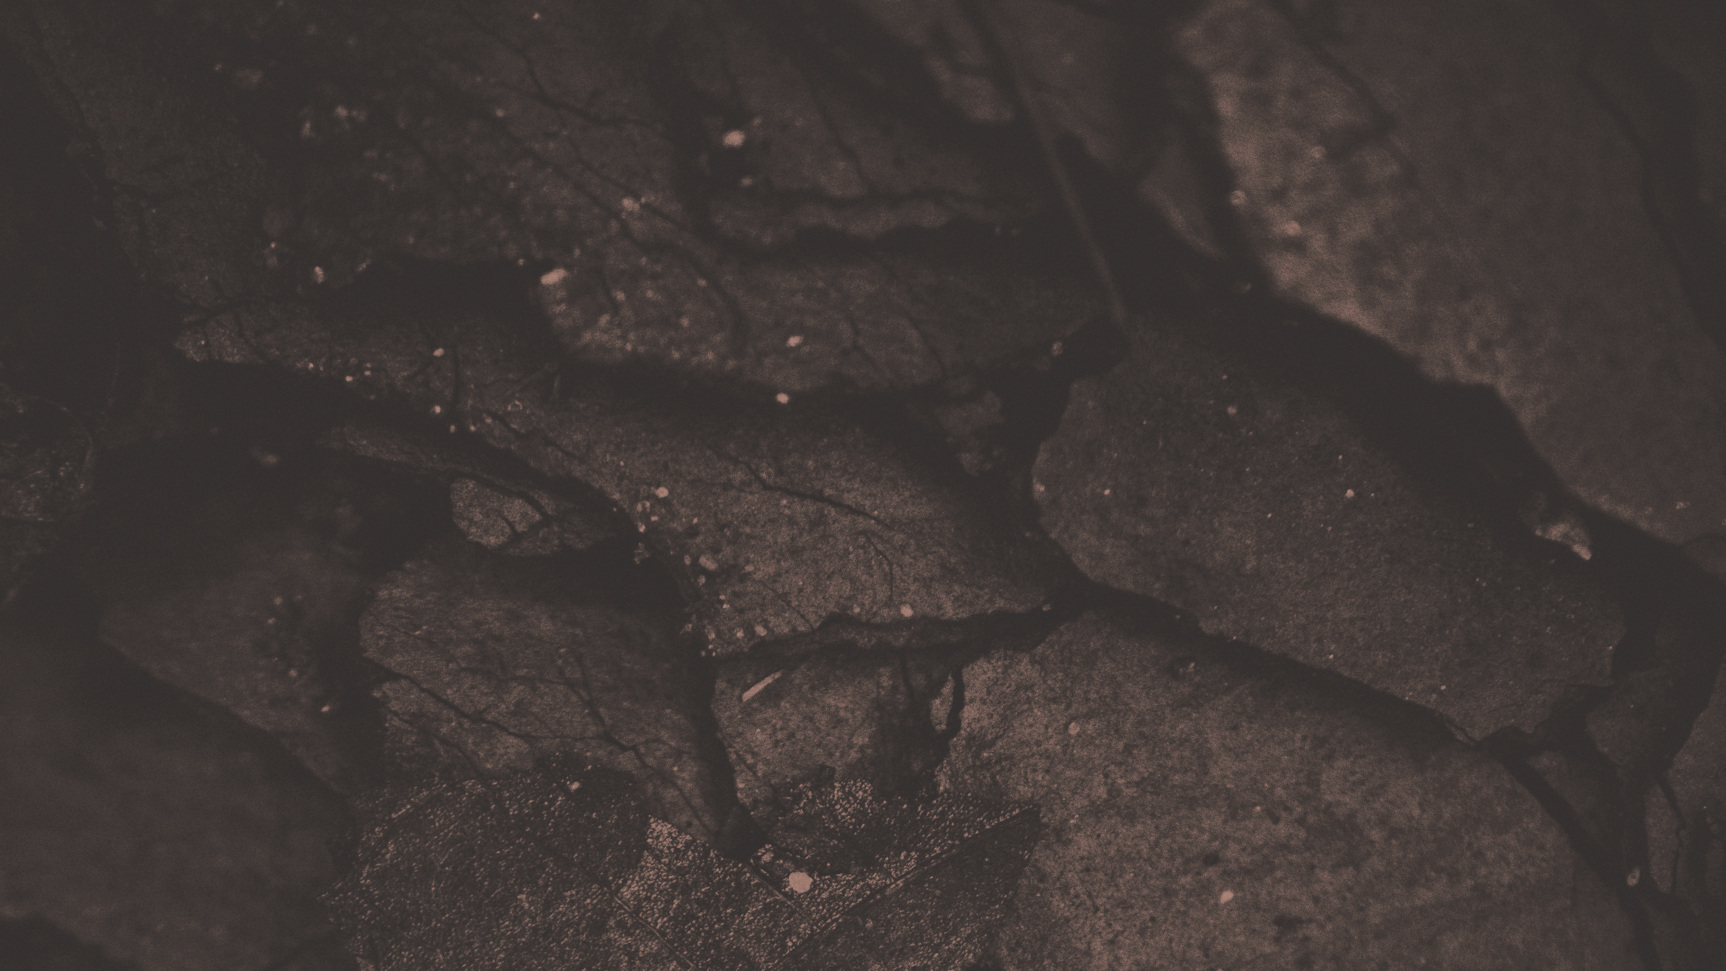
\includegraphics[width=\linewidth]{figures/figure-3a.jpg}
        \caption{}
        \label{fig:3a}
        \vspace{6pt}
    \end{subfigure}
    \begin{subfigure}[t]{\linewidth}
        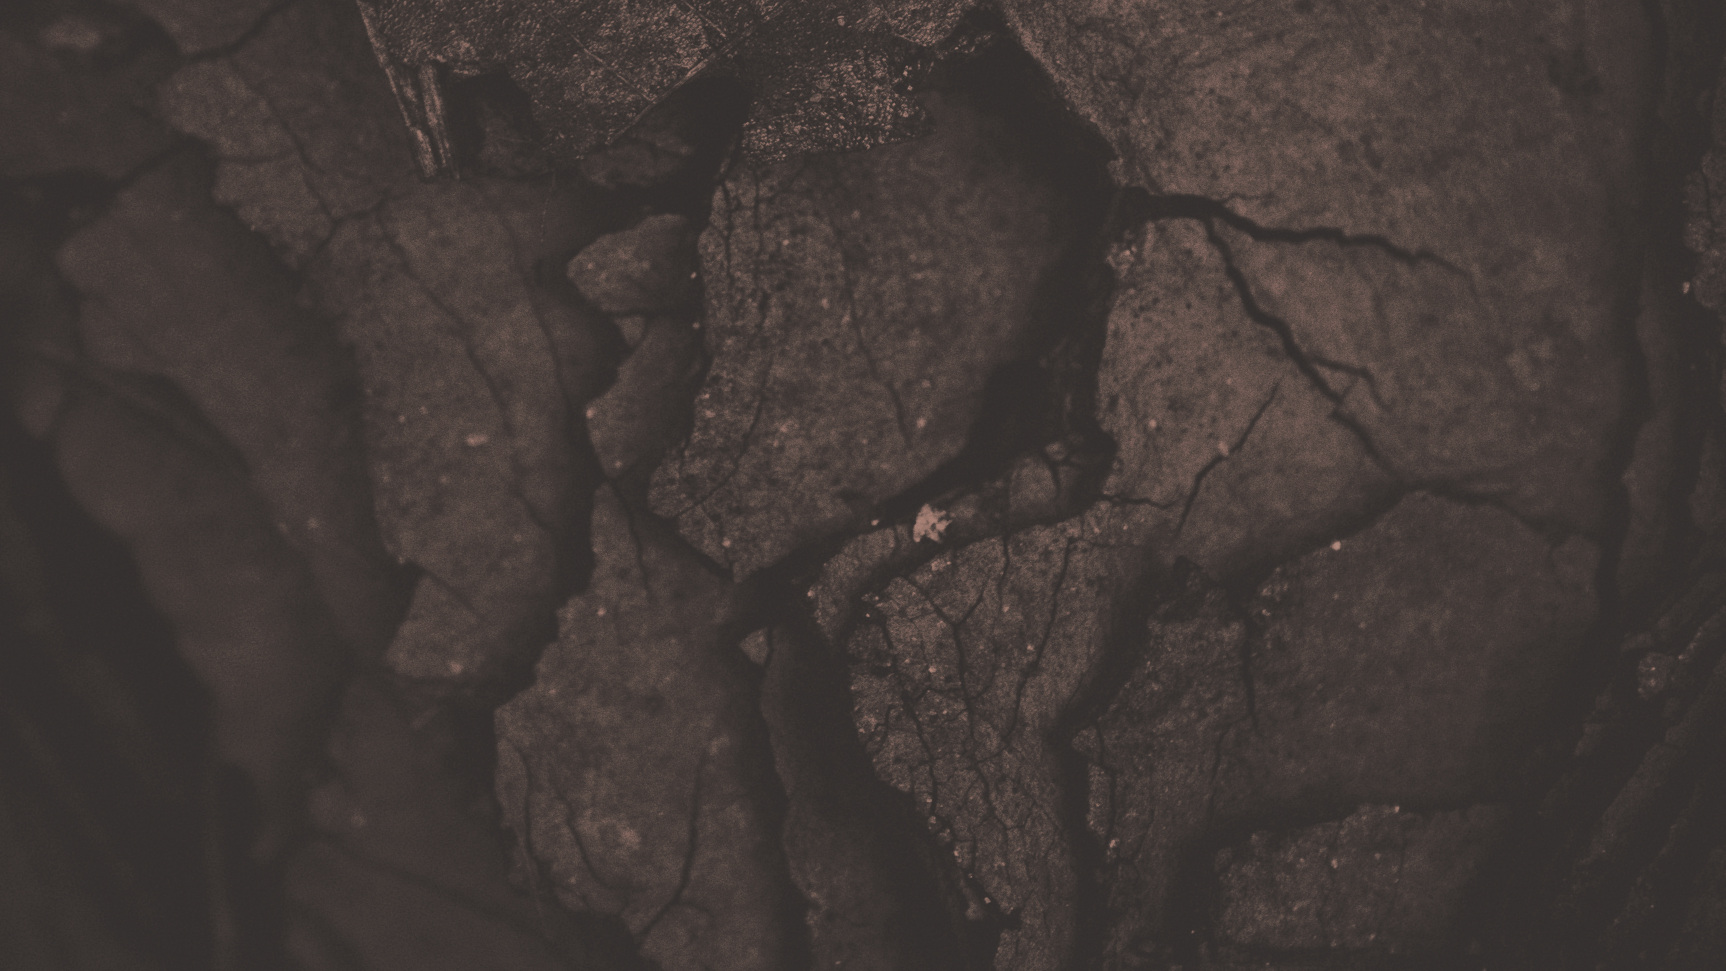
\includegraphics[width=\linewidth]{figures/figure-3b.jpg}
        \caption{}
        \label{fig:3b}
    \end{subfigure}
    \caption{An example of a figure with two subfigures, one appearing above the other. This type of figure is appropriate for combining multiple figures that present similar content or data. (\subref{fig:3a}) First subfigure; (\subref{fig:3b}) second subfigure.}
    \label{fig:3}
\end{figure}

\section*{COMPETING INTERESTS}

It is essential that any and all competing interests—e.g. financial, professional, or personal relationships that are relevant to the submitted work—are declared. If a funding source contributed to the design, data collection, analysis, manuscript writing, or the decision to submit to \textit{Jurnal Rekayasa Proses}, this should be clearly stated. If one or more authors have any form of relationship with \textit{Jurnal Rekayasa Proses} (past or present), the extent of this relationship should be stated. If one or more authors work or have worked for an organization that may benefit from the publication of the article, this must also be clearly stated.

\section*{REFERENCES AND CITATIONS} % Delete this heading and section when typesetting

For the purposes of efficiency and conciseness, aim for 10--25 references, but more are permissible. Use a reference manager such as Zotero or Mendeley to build your reference list, save the file as "references.bib", and then upload it to the \verb|references| folder. Alternatively, copy and paste the contents of the file into the \verb|references.bib| file. All references should be formatted in a manner compatible with BibTeX.

A reference must be cited for it to appear in the reference list. For most cases, you only need to do so as follows. \\

\noindent \verb|\citet{Smith2000}| in the beginning or middle of a sentence: ``\citet{Smith2000} noted that precision is important in science." \\

\noindent \verb|\citep{Smith2000}| at the end of a sentence: ``In science, precision is important \citep{Smith2000}."\\

\noindent If you have cited and formatted your reference correctly, it will automatically appear in the reference list.

\bibliography{references/references}

\atColsEnd{\vfill} % Columns are only balanced after line numbering is disabled

\end{document}